\subsection{Περιγραφή hardware \& κώδικα arduino}
\renewcommand{\figurename}{Σχήμα}
\begin{figure}[htb]
    \centering
    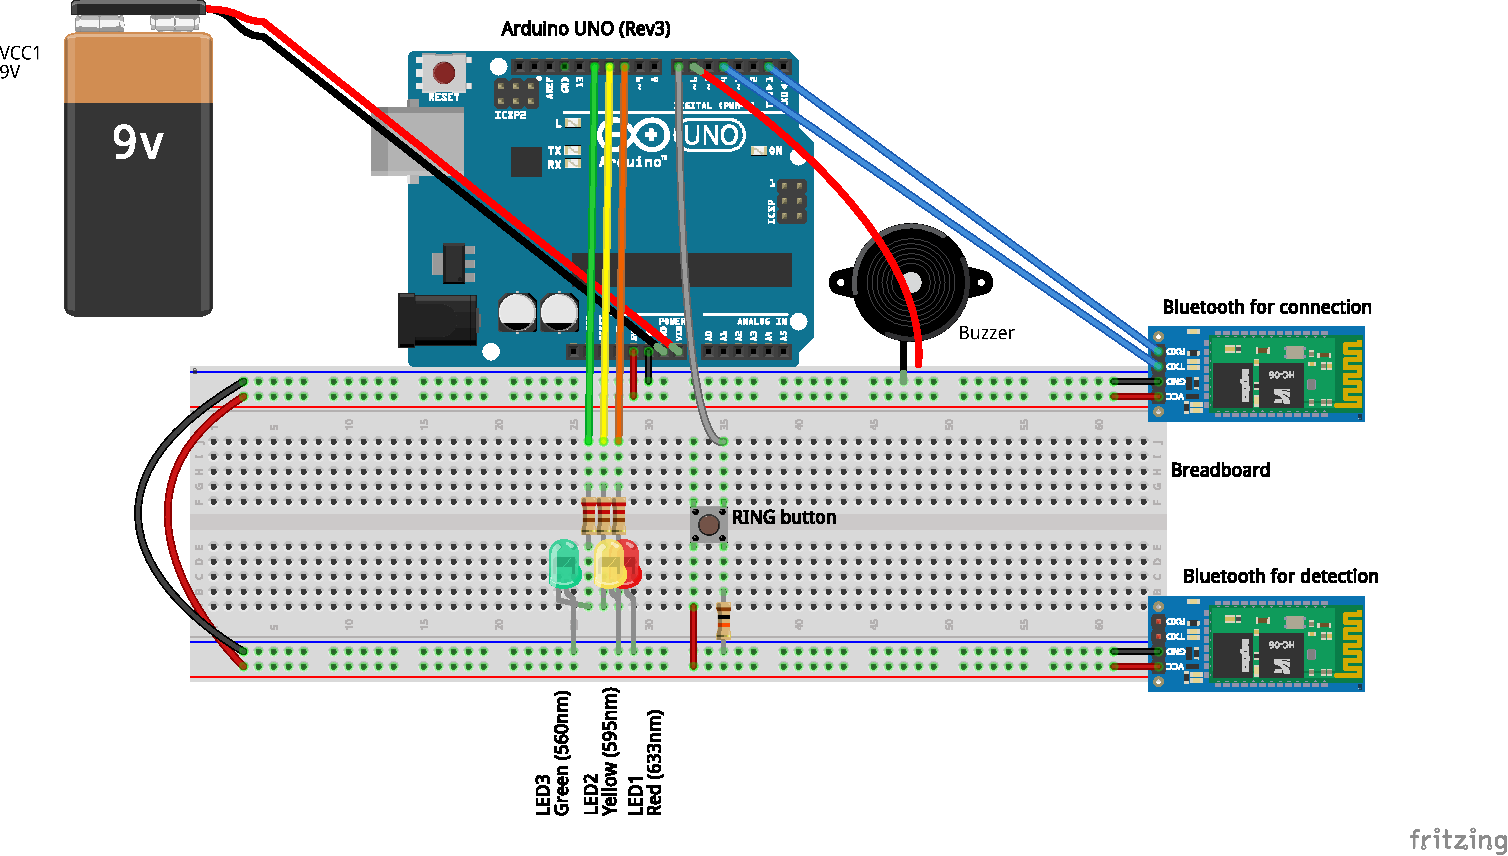
\includegraphics[keepaspectratio, width=\linewidth]{hardware/sketch_bb}
    \caption{Το κύκλωμα που χρησιμοποιήθηκε}
    \label{fig:hardware}
\end{figure}
Με βάση τους παραπάνω περιορισμούς και απαιτήσεις λειτουργικότητας καταλήξαμε στις απαραίτητες αγορές υλικού.
Χρησιμοποιήθηκαν:
\begin{itemize}
\item 1 \href{https://www.arduino.cc/en/Main/ArduinoBoardUno}{Arduino UNO Rev3}:
$1 \times 22 \euro$.
\item 2 HC06 - Bluetooth Module for Arduino:
$2 \times 8 \euro$.
\item 1 breadboard:
$1 \times 4 \euro$.
\item 3 LEDάκια:
$3 \times 0.10 \euro$.
\item 1 μπαταρία \SI{9}{\volt}:
$1 \times 0.80 \euro$.
\item Έναν \href{http://playground.arduino.cc/Learning/9VBatteryAdapter}{9V battery adapter} για arduino:
$1 \times 1.20 \euro$.
\item 1 buzzer:
$1 \times 0.50 \euro$.
\item 1 κομπί:
$1 \times 0.50 \euro$.
\item Καλώδια και αντιστάσεις:
$0.40 \euro$.
\end{itemize}
Σύνολο: $45.7 \euro$.

Στο arduino εκτελούνται όλες οι βασικές λειτουργίες.
Ο κυρίως κώδικας βρίσκεται στο αρχείο \url{Arduino/daerduino/daerduino.ino}:
\begin{itemize}
\item \sloppy Η συνάρτηση \lstinline[language=C++]!bool emergencyButtonPressed()! εκτελείται σε κάθε επανάληψη της κύριας \lstinline[language=C++]!loop()! και αν ανιχνεύσει συνεχόμενο πάτημα του κουμπιού επί τουλάχιστον 1 δευτερόλεπτο επιστρέφει \lstinline[language=C++]!true!.

\item Η συνάρτηση \lstinline[language=C++]!String readBT()! διαβάζει χαρακτήρες από το bluetooth μέχρι να συναντήσει τον χαρακτήρα \lstinline[language=C++]!';'!.

\item \sloppy Η συνάρτηση \lstinline[language=C++]!void interruptBluetooth()! καλείται σαν timer interrupt
κάθε \lstinline[language=C++]!INTERRUPT_FREQUENCY_MICROS! \si{\micro\second}
και στέλνει στη συνδεδεμένη συσκευή android τον χαρακτήρα \lstinline[language=C++]!"C"! ώστε να επιβεβαιωθεί η σύνδεση και διαβάζει τις εντολές που στέλνει η συσκευή android.
Οι διαθέσιμες εντολές είναι:
\begin{itemize}
\item \lstinline[language=C++]!"RING"!: ενεργοποιεί το alarm: \lstinline[language=C++]!playRing = true;!.
\item \lstinline[language=C++]!"RSTOP"!: απενεργοποιεί το alarm: \lstinline[language=C++]!playRing = false;!.
\item \lstinline[language=C++]!"POFF"!: απενεργοποίηση προστασίας.
\item \lstinline[language=C++]!"PON"!: κατάσταση προστασίας.
\item \lstinline[language=C++]!"SEMI"!: κατάσταση ημι-κινδύνου.
\item \lstinline[language=C++]!"DANG"!: κατάσταση κινδύνου.
\end{itemize}

\item Η συνάρτηση \lstinline[language=C++]!void updateLEDs()! διαχειρίζεται τα LEDs ανάλογα με την τρέχουσα κατάσταση.

\item Η συνάρτηση \lstinline[language=C++]!void updateLEDs()! διαχειρίζεται τα LEDs ανάλογα με την τρέχουσα κατάσταση.

\item Η συνάρτηση \lstinline[language=C++]!void loop()! είναι η κυρίως λούπα της εφαρμογής, αναλαμβάνει:
\begin{itemize}
\item Το reset του watchdog.
\item Την αναπαραγωγή του alarm μέσω της \lstinline[language=C++]!sing()! εάν η \lstinline[language=C++]!alarmShouldPlay()! επιστρέψει \lstinline[language=C++]!true!.
\item Την αποστολή της εντολής \lstinline[language=C++]!"RING"! στην συσκευή android σύμφωνα με την επιστρεφόμενη τιμή της \lstinline[language=C++]!emergencyButtonPressed()!.
\end{itemize}
\end{itemize}

Στο \url{Arduino/daerduino/supermario.ino}
βρίσκεται η συνάρτηση \lstinline[language=C++]!sing()! που αναλαμβάνει την αναπαραγωγή του alarm στο buzzer.
